\documentclass[12pt]{article}

\usepackage[english]{babel}
\usepackage[utf8x]{inputenc}
\usepackage{pdfpages}
\usepackage{lastpage} % Required to determine the last page for the footer
\usepackage{extramarks} % Required for headers and footers
\usepackage{graphicx} % Required to insert images
\usepackage{listings} % Required for insertion of code
\usepackage{courier} % Required for the courier font
\usepackage{color}
\usepackage{grffile}
\usepackage{float}

\usepackage[a4paper, total={6in, 8in}]{geometry}

% Margins
\topmargin=-0.45in
\evensidemargin=0in
\oddsidemargin=0in
\textwidth=6.5in
\textheight=9.0in
\headsep=0.25in
\fboxsep=0mm%padding thickness
\fboxrule=2pt%border thickness

\linespread{1.1} % Line spacing

\newcommand{\Title}{Software architecture document} % Assignment title
\newcommand{\Class}{COS\ 301 Final year project} % Course/class
\newcommand{\pd}{Post-Doctoral}
\newcommand{\ssr}{Soft\color{green}{Serve }\color{black}}
\newcommand{\version}{3.0 (Final)}
\newcommand{\iteration}{6}
\newcommand{\client}{Ms. Cathy Sandis (UP DRIS)}
\newcommand{\project}{Post-Doctoral management System}
\newcommand{\repo}{https://github.com/mox1990/Project-Postdoc.git}
\begin{document}

\vspace{4em}

\begin{center}%

\begin{figure}[ht!]
\centering

\includegraphics{../Images_Docs/logo.png}
\end{figure}
\LARGE \bf \Class \\[0.25em]
\LARGE \bf \project \\[1em]
\LARGE \bf \Title \\[0.25em]
\large \bf \today\\
\bf Version \version\\
\bf Iteration \iteration\\[0.5em]
\Large \bf Prepared for \client\\
\Large \bf by
\Large {\bf \ssr Group }\\[0.5em]
\LARGE {\bf Group members}\\[0.25em]
\large
Kgothatso Phatedi Alfred Ngako (12236731) \\[0.5em]
Tokologo “Carlo” Machaba (12078027) \\[0.5em]
Mathys Ellis (12019837) \\[8em]

\end{center}%

%\newpage
%{\LARGE \bf Change log}\\[2em]

\begin{center}
\begin{tabular}{|l|p{1.4cm}|p{8cm}|p{2.8cm}|}
\hline
\multicolumn{4}{|c|}{\bf Change log} \\
\hline
 Date & Version & Description &  Person \\
\hline
03/10/2014 & v 0.0 & Combined architectural specification and architectural requirements specification & Mathys Ellis \\
\hline
03/10/2014 & v 1.0 & Complete restructuring and most of the editing and additions  & Mathys Ellis \\
\hline

%\end{tabbing}
\end{tabular}
\end{center}
\newpage
\tableofcontents

\listoffigures
\newpage
\section{Project Repository}
\textbf{\repo}
\newpage
\section{Document description:}


\subsection{Document purpose:}
\vspace{0.2in}
The Software architecture document provides the architectural requirements that the project will need to follow as well as a set of quality requirements that must be met by the system. The quality requirements have been quantified in order to provide the SoftServe group and the client with a means to test the system for non-functional compliance. This allows the SoftServe group to set up tests in the non-functional testing document that can be used at the end of the development cycle to verify that the system complies with the architectural and quality requirements specified by this document. Further the document provides the architecture specification which covers architectural descriptions of various architectural factors that the project will need to follow when developing the system.  Architecture in this document's context refer to the technological basis and software development and organisational styles and strategies of the project. Thus this document serves as a contract between SoftServe and the client, Mrs Cathy Sandis of the DRIS of the University of Pretoria in terms of what technologies the project should incorporate as-well as the software development infrastructure that the system will be based on and also the quality the system should be of once the project is complete.
\vspace{0.2in}

\subsection{Documentation methodology}
\vspace{0.2in}
\begin{flushleft}
The documentation and software development methodology used by the project adhere to the guidelines set out by the scum agile methodology. Thus this document has undergone and will undergo various iterations that may extend or reduce the contents of the document.\\

This document was created using various insights gained throughout the COS 301 course and the requirement elicitation techniques and definitions as specified by Klaus Pohl’s book Requirements Engineering: Fundamentals, Principles, and Techniques [Dr.Phol, K., 2010].
The quality requirements and aspects of the architectural requirements, were elicited from the following sources:
\begin{itemize}
	\item Numerous interviews with the client.
	\item On-line research into UP Post doctoral applications.
	\item Correspondence with the UP IT department.
	\item Collecting and analysing various documents such as:
		\begin{itemize}
			\item The initial project request document
			\item Application forms
			\item Renewal forms
			\item CV templates
			\item Approval and recommendation forms
		\end{itemize}
\end{itemize}
\end{flushleft}	

\vspace{0.5in}

\subsection{Document conventions:}
\vspace{0.1in}
\begin{itemize}
\item Documentation formulation tool: LaTeX
\end{itemize}

\vspace{0.2in}

\subsection{References:}
\vspace{0.1in}
\begin{itemize}
\item Kang, A. August 9, 2002, \textit{Enterprise application integration using J2EE}, Available from: http://www.javaworld.com/article/2074488/enterprise-java/enterprise-application-integration-using-j2ee.html , [Accessed on: 17 May 2014]
\item Ali Babar, M., \textit{Architectural Patterns and Frameworks, Week 3, Lecture 3},Available from: https://blog.itu.dk/MSAR-E2013/files/2013/09/wk3\_lect3\_patternsframeworktactics.pdf, [Accessed on: 21 May 2014]
\item Dr.Phol, K., 2010, \textit{Requirements Engineering: Fundamentals, Principles, and Techniques}, Springer, Heidelberg.
\item Kayal, D., 2008, \textit{Pro Java EE Spring Patterns: Best Practices and Design Strategies Implementing Java EE patterns with Spring Framework}, Apress, New York.
\item Jendrock E, Cervera-Navarro R, Evans I, Haase K, Markito W, \textit{The Java EE 7 Tutorial}, Available from: http://docs.oracle.com/javaee/7/tutorial/doc/home.htm , [Accessed on: 20 May 2014]
\item Oracle. April 2014, \textit{The Java EE 7 Tutorial}, Available from: http://docs.oracle.com/javaee/7/tutorial/doc/overview.htm , [Accessed on: 20 May 2014]
\end{itemize}	

\vspace{0.5in}

\newpage
\section{Architecture requirements}

\subsection{Architectural Scope}
This section discusses the architectural scope that the software architecture of the system must cover in order to produce a compliant system:
\begin{itemize}
\item A persistence infrastructure using a DBMS to facilitate the storage of the various domain objects (e.g CVs, DRIS information, and Applications). So to allow the system to store and centralise the various data that the system will be handling as outlined in the functional requirements and application document.
\item A multi-user session infrastructure to assist in realizing the security requirements of authenticating users and their actions.
\item A work-flow infrastructure for processing applications that can be modified and extended. 
\item A RESTful web service infrastructure, to provide a means for the system to be integrated in other systems and also to allow lightweight data communication between the users and the server and support for mobile platforms. 
\item A report generation infrastructure in order to support the data retrieval requirements of the client.
\item An email infrastructure for the system to use in order to provide notification support.
\item A action logging infrastructure to track user activity on the system, in order to provide audit-ability.
\item A gateway infrastructure to provide access control to services provided by the system.
\item A pre post condition infrastructure to dynamically change per and post conditions for certain operations in the system.
\end{itemize}

\newpage
\subsection{Access channel requirements}
\vspace{0.2in}
The only two access channel requirements specified by the client are as follows:
\begin{itemize}

\item \textbf{All stakeholders:}
Users of the system will access it through the HTTP and HTTPS protocols either via a web browser client or some software, which makes use of the Restful API the system provides. Both will be locally installed on a user's desktop or mobile platform. Web browsers are expected to be HTML 5 compliment. This access channel will provide excellent availability and usability of the system due to the RESTFul nature of most internet enabled systems and the ease of using web browsers. The access channel will allow different stakeholders access to different sections of the system based on the roles assigned to their accounts. 

\item\textbf{System Administrator:}
The system administrator will require the same as the above but will in addition need to be able to conduct any external administration duties on the system which can not be done via the the above access channel. Such as updates, server maintenance, etc. Thus such operations will be done via the server by some terminal emulation protocol, such as Telnet or SSH, or by physical access. 

\end{itemize}
\vspace{0.2in}

\subsection{Quality requirements}
\vspace{0.2in}

These are the quality requirements as specified by the client and are also in the order of precedence. Where the first takes the highest precedence.

\subsubsection{Usability requirements}

\begin{flushleft}

This is first and foremost quality requirement stipulated by the client. The primary language of the system will be South African English. Any other language support is not considered part of the requirements but the system will be designed to allow for such development in the future.\\

\vspace{0.1in}

The system's UI will only consider 2 types of user categories with regard to usability:

\begin{itemize}

\item\textbf{Trained user:}

This type of user will have to have training in understanding how the system functions and how to use it. Their computer skills will be assumed to be in the range of basic to intermediate. Thus the user interface can allow for certain complexities but these complexities must be kept at a minimal. These user will be regarded as system administrators or specialised users of the system. The stakeholders who fall under this category is the DRIS staff members overseeing the application process and any technical or maintenance support users.

\item\textbf{Normal user:}

This type of user will have no training with regard to the system. Their computer skills will be assumed to be none or minimal. Therefore the UI that they will have access to will be simplistic and will be as user friendly as possible. The stakeholders that fall under this category will be Prospective fellows, Research fellows, Referees, Grant holders, HODs, Dean's office members and Post-doctoral committee members.

\end{itemize}

In order to quantify the above the SoftServe group will need to provide the system with a uniform user experience that is as simplistic and as visually oriented as possible without negating the below requirements severely. In addition to this any form of help text or instruction should be written in as natural, uncomplicated and unambiguous manner as possible. 

\end{flushleft}

\subsubsection{Security requirements}

\begin{flushleft}

The system will need to be fully secured since it deals with confidential information such as person information, application statuses, financial data and meeting information. Also since the systems main goal is to provide stable and audible application and renewal process flow the system may not be vulnerable to data tampering or any tampering whatsoever. It should be noted that this requirement conflicts with the Usability requirement above as it is known that the more secure a system becomes the less user friendly it becomes. Therefore the SoftServe group will try to balance the two requirements in such a way that neither of the two is negated.\\
\vspace{0.1in}

The system will have to provide different security roles to the registered users on the system. Any number of roles should be assignable to any user by a system administrator to allow for flexibility.\\
There will also need to be predefined roles so to allow a stakeholder from list of stakeholders in the vision and scope document, to only have the ability and access to perform the actions as defined by the vision and scope document.\\
The system administrator should be able to access all the sections in the system and should be able to modify them except where only the system itself has that right.\\
Another security requirement is that the audit trail must not be allowed to be modified by any human user and only allow the system to be able to insert data into the audit log. Further the audit table should only allow be query-able by a user with the correct security role.\\
To further quantify this requirement the system must provide some means of a centralised user authentication that acts as a gateway for all users of the system. Also every time some action is made by the user the user needs to be re-authenticated to insure that the user does have the correct privileges and if any user account changes where made it takes immediate affect. \\
Any form of account retrieval token or on-demand user account creation tokens must expire within a specified time period. For account retrieval token this should be 1 hour. For on-demand user account creation this should be about 2 days.

\end{flushleft}

\vspace{0.1in}

\subsubsection{Auditability:}

\begin{flushleft}

This is seen as the third most important requirement according to the client. The system needs to provide some form of an audit trail of all critical actions that occur in the system. Critical actions are considered: user account management operations, login action, logout action as well as any operation by a user that leads to a change in the data stored by the system. The Audit trail will be in the form of a read-only table stored in the database as stipulated in the security requirements above.\\

To quantify this requirement, the system will need to have an active audit log that can capture all the actions, that meet the list of critical actions, of each user that uses the system. With regards to usability, the feature needs to run in the background and not be noticeable by any user while they are using the system except if it is deliberately queried.

\vspace{0.1in}

\end{flushleft}

\subsubsection{Scalability requirements}

\begin{flushleft}

As research is still viewed as small field that is slowly growing by the client this is only the fourth most important requirement for the system. The current aim is to create a scalable system that can support 50 to 500 applicants per year with possible growth to a 1000 or more. This is in line with the figures given by the client and the growth, over the next ten to twenty years, in the research sector of the University of Pretoria.\\
\vspace{0.05in}

The system needs to be scalable in regard to the following factors:
\begin{itemize}

\item\textbf{Performance:} This aspect of the system regards the speed and responsiveness of the system.
The system needs to be handle large report queries in less than 10 seconds. It should be able to handle any application approval service processing in less than 3 seconds. It should be able to send emails instantly from the system side. Note this may be difficult to measure due internet bandwidth and receiving mail server constraints. Login, logout and user authentication should be handled in less then a second by the system this does not  considering the transfer of data to and from the server which is depended on the network connection speed.\\

\item\textbf{Storage:} This aspect of the system regards the growth and shrinking of the data that is stored by the system.
The system will need to be able to handle a database that is in the range of 1 GB to 15 GB that has the potential to grow even larger. The reason for this stems from the fact that the system will need to store a large amount of active data over a period of about 3 to 8 years before it can be archived.
\\Another requirement of the system is that it will need to support archival functionality and archived data that will eventual store all the old data from the active database for as long as time period as possible. Since the archival database should only grow it will need to be about 15 times larger than the active database. Due these reasons the calculation of how much space should be required will only be possible once the system is implemented and practically tested.\\The suggested linear formula to the above analysis is as follows: 
\begin{equation}
A \times ( (Xna \times Nna) + (Xra \times Nra) ) = B
\end{equation}

A = Number of years for which archival or active support is intended\\
B = Number of bytes needed on average for A years\\
Xna = Average number of bytes per new application\\
Xra = Average number of bytes per renewal application\\
Nna = Number of new applications a year\\
Nra = Number of renewal applications a year\\

\item\textbf{Concurrency:} This regarded as the amount of active users on the system at the same time.
The system will need to support at least 100+/- concurrent users efficient and effectively since the system requires multiple stakeholders to part take in the application process while there can be multiple applications occurring at the same time.\\

\end{itemize}
\end{flushleft}
\vspace{0.1in}

\subsubsection{Availability:}

\begin{flushleft}

The system's availability on designated networks will depend on the availability of the University of Pretoria's servers or whatever hosting service that will used to host the system. It should be noted that the former will only be possible if the project is considered acceptable by the UP's IT department.\\
In order to quantify this it should be seen as follows: If the hosting service's servers hosting the system are active and provide access over a designated network then the system must be available over that designated network. Where the designated networks are defined as the internet and/or the local network where in the server of the hosting service is located.

\end{flushleft}

\vspace{0.1in}

\subsubsection{Testability:}

\begin{flushleft}

The system must be testable. This will be done using unit testing and following the test plan that will be laid out in the testing document of this project.\\

\vspace{0.1in}

Unit testing will test each unit in regard to:
\begin{itemize}

\item\textbf{Preconditions}
\item\textbf{Post conditions}

\end{itemize}

The project will also have two phases of testing:

\begin{itemize}

\item\textbf{Offline:} This is the initial phase of testing and debugging which will be done with pseudo data.
\item\textbf{Online:} This is the final phase of testing and debugging which will be done with active real time data.

\end{itemize}

\end{flushleft}

\vspace{0.1in}





\vspace{0.1in}	



\vspace{0.2in}

\subsubsection{Robustness:}

\begin{flushleft}

This requirement was identified by the SoftServe group as being very important since the system will be receiving and handling large amounts of sensitive data. Thus the integrity of the data must be insured. To do this the system needs to be robust in in terms of its data storage routines, security routines and data validation, system integrity. 

These four aspects of robustness are quantified as follow:
\begin{itemize}
\item \textbf{Data storage}: When data is stored the data needs to be validated against a set of storage rules and constraints. Many DBMS packages allow this type of validation through data typing and allowing the database administrator to a specify constraints.
\item \textbf{Security}: As mentioned above in the security requirements the re-authentication of users is required and any form of account retrieval token or on-demand user account creation tokens must expire within a specified time period and that as only one token may be active at a time.
\item \textbf{Data validation}: All data that is manually imputed by a user, such as text, numbers, emails, passwords, etc. Must be checked to see if they meet constraints imposed on them through the use of data type checking and regular expression analysis. Any section in the system that requires certain data to completed before performing a action must be checked for completeness before allowing the user to perform the action. Where completeness means the data is not empty and validate according to constraints imposed on it.
\item \textbf{System Integrity}: If there are any defects with any other components with in the system and a task cannot be completed the user will also be notified immediately with the appropriate message sent to them.
\end{itemize}


\end{flushleft}

\vspace{0.1in}

\vspace{0.2in}

\subsubsection{Flexibility:}

\begin{flushleft}

The system is designed in such a way that adding new features can be done without extensive code restructuring. The process of adding new features will require the programmer to create a new module for the new functionality.

\end{flushleft}

\vspace{0.1in}

\vspace{0.2in}

\subsubsection{Reusability:}

\begin{flushleft}

The System's components will be used again where applicable. The Login credentials is an example of areas where the system will be reused.

\end{flushleft}

\vspace{0.1in}

\vspace{0.2in}

\subsubsection{Maintability:}

\begin{flushleft}
The system administrator will have the responsibility of adding updates that a programmer may wish to add to the system. 

\end{flushleft}

\vspace{0.1in}

\vspace{0.1in}

\newpage
\subsection{Integration requirements}
\vspace{0.2in}
The client's primary integration requirement is to completely integrate with UP's PeopleSoft management system. With the regards the vision and scope document it should be noted that the knowledge the SoftServe group has of the Peoplesoft system is very limited due to UP's IT department's prerequisite for the project. The system has to integrate with the PeopleSoft as follows:

\begin{itemize}
	\item Must be able to create exportable data packages containing the information of prospective and current research fellows that can easily be loaded into the PeopleSoft system or used by other parties. In terms of quality requirements:
	\begin{enumerate}
		\item \textbf{Performance:} The system should be able to handle the export and importing of application information at a reasonable rate of about at least 10 full application data packages in a second. The system should be able to import and generate on-demand user accounts at a rate of 50 per second. For exporting it should be able to do so at 60 accounts per second.
		\item \textbf{Scalability:} The system should be able to export or import as much data as specified by the user as long as it does not exceed the size of the database or the size of users secondary storage. 
		\item \textbf{Audibility:} Any export and import should be recorded by the system.
	\end{enumerate}  
	\item Must be able to query PeopleSoft system to retrieve the account information of internal individual or group Stakeholders to create a uniform login experience. As specified by the vision and scope document this will not be possible at the time of writing since no API can be given to the SoftServe group. 
	\item To standardise information the following is to be done:
	\begin{enumerate}  
		\item Must assign Prospective fellows with a id number in such a way that is integrable with UP Emplid. SoftServe suggests: "f" + 8 digit code.
		\item Stakeholders that have a Peoplesoft account must use their UP emplid id as a user name. The password may vary.
		\item Must be able to provide access to the NRF researcher ratings list but not utilize it as the client has stipulated human error is possible in maintaining of those ratings.
	\end{enumerate}
\end{itemize}

SoftServe has also decided to add two further integration requirements in an attempt to improve future integration with other systems and to improve the application process. The two requirements are as follows:

\begin{itemize}
	\item \textbf{RESTful API/Web services} - The system will need to be able to provide a set of RESTful web services that is able to make use of all the back-end services provided by the system. This will allow future systems to easily integrate with other systems who wish to make use of the system. The interchange formats for the data should be limited to XML and JSON as these are the most universal and at the time of writing the de facto data formats. This will also help solve any future integration with the PeopleSoft system.
	\item \textbf{Google Scholar} - The system will need to be able to integrate with the Google Scholar services. The service needs to allow the system to be able to create full fledged queries for google scholar and be able to retrieve their results. This will be used to allow applicants to quickly populate their CV references by having the system quick search google scholar. There is unfortunately at the time of writing no such API. Therefore the SoftServe group will need to create our own API. This proposed by employing a HTML scrapping technique. 
\end{itemize} 

\vspace{0.2in}

\subsection{Architecture constraints}
\vspace{0.2in}

The following architecture constraints have been selected by SoftServe group as being suitable for the system. Please note due to the client's inexperience with software development and the technologies that exist she has allowed the SoftServe group to use their expertises, to decide on the appropriate set of architectural constraints that can meet the above requirements.
\begin{enumerate}
\item Database technology: MySQL
\item Programming paradigm: Object-Oriented
\item Programming language: Java
\item Development platform: Java-EE 7 
\item System architecture: Java-EE
\item Architectural frameworks: JSF, Java Persistence API, JAX-RS
\item Architectural pattern: Layered (Multi-tiered)
\item Development technologies: EJB, JSP, Expression Language, JDBC, JTA, Java EE Connector Architecture, JAF, JavaMail, JNDI, Concurrency Utilities for Java EE, JAXB, PrimeFaces
\item IDE: Netbeans 8.0
\item Build environment: Apache Maven 3
\item Web server software: GlassFish 4.0 server
\item Web interface protocol: HTTPS
\item Client web browser: Microsoft Internet explorer 9+, Google Chrome 30+, Mozilla FireFox 20+, Opera, Safari
\item Client device operating systems: Windows, iOS, Android, Linux.
\item Proprietary software: Cannot make use of this due to financial constraints. 
\end{enumerate}
\vspace{0.5in}


\section{Architectural Patterns and Styles} % skipped till further notice.
This section describes the various architectural patterns that will be employed by the project. It should be noted some of these patterns are implicitly employed by the system due to the development approach.  

\subsection{Layered pattern}
The system will explicitly employ a multi-tier/layered architectural pattern to form what is known as the Java Enterprise Edition system architecture. This will allow the client(s) to be decoupled from the server. This pattern is widely used and provides various benefits. Some benefits include modularity, encapsulation, re-usability of components, decoupling, system maintainability, pluggable-ness of layers and complexity reduction [Ali Babar, M.] [Oracle, 2014][Kayal, D., 2008]\\
\\
The Java EE system architecture is designed to support highly scalable, distributed, transactional and portable applications that use the speed, security, and reliability of a Java EE server to provide powerful enterprise applications. [Oracle, 2014] For this reason SoftServe believes this system architecture is well suited for the development of the Post-Doctoral management system as it will satisfy the requirements in terms of quality and functional as stipulated by the client. The following diagram provides the system architecture that will be employed by the system:\\

\begin{figure}[H]
\centering
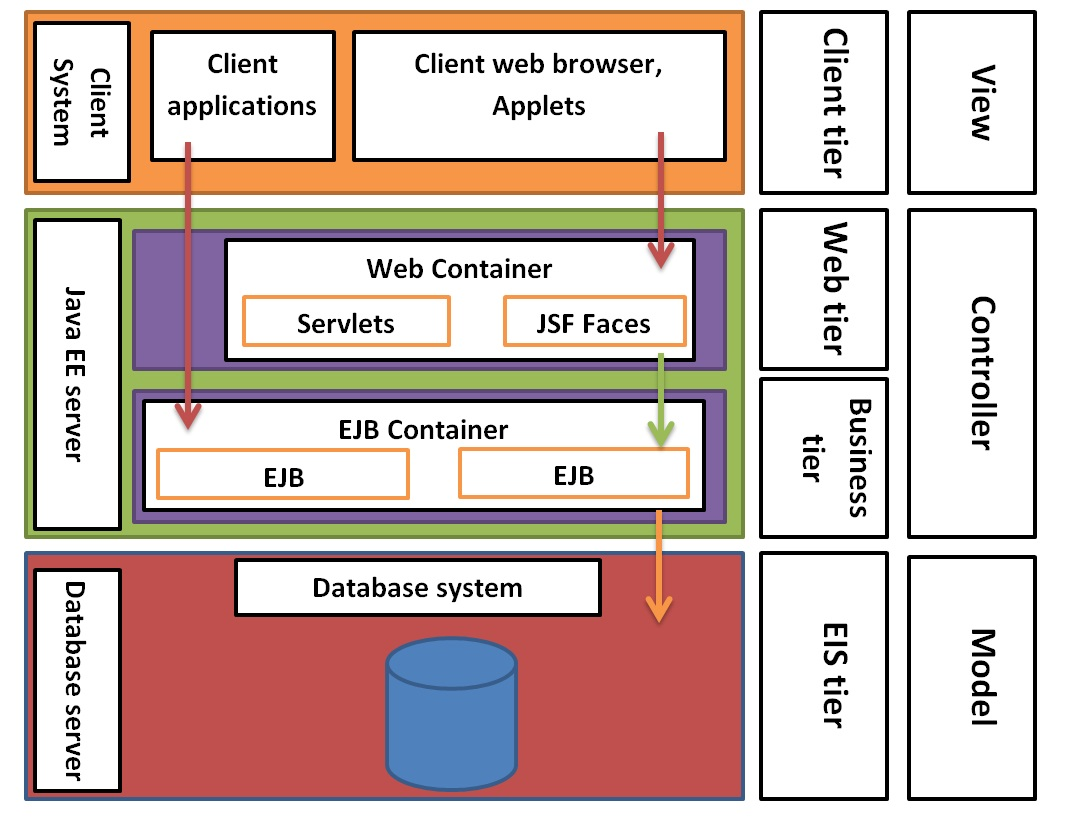
\includegraphics[scale=0.6]{../Images_Docs/Diagrams/Architecture/Java EE system architecture.jpg}
\caption{Java EE system architecture with respect to the Post-Doctoral management system}
\end{figure}

\subsubsection{Client layer}
This layer runs on the client system and encapsulates the various components that a client system may use to access the Java EE server-side layers. These components include dynamic web pages, Java applications and Java applets. In order to make the Post-doctoral application management system accessible to any stakeholder over the internet and provide a uniform user experience the system will make use of the JSF frame work to provide web pages via a web browsers and RESTful web-services to provide access to the system via other client side applications. [Oracle, 2014]  

\subsubsection{Web layer}
This layer runs on the Java EE server and hosts the Web container and RESTful web services. It provides the management and web page generation support for the web pages that the system has to provide to the client Tier through the use of of the Java ServerFaces Facelets and backing beans. It also facilitates the communication between the business layer and client layer and thus handles the data validation and transformation required by such communication.[Oracle, 2014] 
\subsubsection{Business layer}
This layer also runs on the Java EE server and hosts the Enterprise Java Bean container. It provides the business logic section for the Java EE application in the form of Enterprise Java Beans which are simply classes of POJOs that represent various persistence entities of the persistence layer, system messages, sessions, services. It also hosts any auxiliary services that the application wishes to implement in order to help the EJBs. This layer communicates with EIS layer in order provide access to the database and various other lower level infrastructures that the Java EE application requires. [Oracle, 2014]

\subsubsection{Enterprise Information/Persistence layer} 
The EIS layer provides mainly the support for database systems that are used by the Java-EE application. This layer can run on the Java-EE server as a virtual server or on a physically different database server. Due to the project budget and technical constraints the former will used by the system. [Oracle, 2014] 

\subsection{MVC Pattern}
This pattern is implicit due to the design of the JSF framework and the Java-EE layers. The JSF framework is built according to the MVC pattern. And for case regarding Java-EE, the layers can be grouped as into the 3 different components of the MVC pattern as follows:

\subsubsection{View}
The view is what is presented to the user and is the front-end of the system. Thus this is the Client layer in Java-EE and is the face-lets in JSF. This component makes use of the controller in order to provide information to the user and send information to the Model.

\subsubsection{Controller}
The controller is the controlling mechanism of the system and provides the functionality and business logic of the system. Thus this encapsulates the Web layer and EJB layer of Java-EE as they provide the data conversion and business logic of the system. In JSF this is the backing beans.

\subsubsection{Model}
The Model is the data storage component of the system and provides the mechanisms necessary to store data and use it for use by a system. Thus this represents the EIS/Persistence layer in Java EE as it deals with the data stores. In JSF this is the persistence layer.

\subsection{Pipes and Filters}
This pattern is a consequence of the layered pattern employed by the system. Since the data that passes from layer to layer is encapsulated by a logical pipe which is the path of the data flow in the system. In this pipe the layers and the operations within the layers which the data flows through acts as filters as they may add or remove data from the objects passing in or add or remove inputs to the next layer or operation.\\
The application work flow can also be  seen as a pipe and filter which is bidirectional. Where the pipe is the process flow and the filters the stages in the work flow. It is bidirectional since the applications can move forward and backwards through the work flow.  
%%%%%%%%%%%%%%%%%%%%%%%%%%%%%%%%%%%%%%%%%%%%%%%%%%%%%%%%%%%%%%%%%%%%%%%%%%%%%%%%%%%%%%%%%%%%%%%%%%%%%%%%%%%%%
\section{Architectural Tactics and Strategies} % skipped till further notice.
This section describes the architectural techniques which will be used in order for the system to satisfy the quality requirements. 

\subsection{Concurrency/Spreading work load}
The Java Platform offers support for concurrent programming, which is the basis for implementing many of the services offered by Java EE containers via concurrency utilities. This is realized through the use of thread pooling, threads, queuing and scheduling strategies.(Cervera-Navarro, Evans, Jendrock, Haase and Markito 2014).\\

\subsection{Exception handling}
To improve the robustness and reliability of the system the system employees various usages of try catch control structures and exception classes. This helps prevent system failure and improves availability. Also user friendly messages will be displayed to users using a messing framework to notify users about system failure or exceptions.

\subsection{Logging}
To improve security, audibility, reliability and maintainability the system logs exceptions and various other information such as queries and system status on a server log for later review. Thus it can be used to pinpoint bugs or attacks.

\subsection{Testing framework}
In order to satisfy reliability a testing framework will be used by the system in which unit and integration tests are designed and automatically ran at build time. To complement this a mock frame work will also be used to mock out dependencies for unit tests.

\subsection{Checkpoints and roll-backs}
To prevent the data integrity from being compromised when storing various items to the database in single operation the system will make use of two-phase commits and a entity manager that will only commit in a single transaction once all the data has been created/removed/modified in the temporary entity graph. Thus if an error occur all changes are rolled back to the previous checkpoint.

\subsection{Maintaining backups}
To improve reliability of the system the system will allow for full backups of the entire working database to be created.

\subsection{Interceptors}
To improve security and audibility interceptors will be employed by the system to detect the execution of methods that are demarcated by appropriate annotations. These interceptors will process the inputs to see if the user can use the service or if it needs to be logged by system in the working database. Further they will be used to improve maintainability by checking pre and post conditions of demarcated functions.

\subsection{Minimize access channels}
Another step taken to improve the security of the system was to minimize the access channels to only that of the web browser interface and RESTful API. Thus allowing the focus of security implementations on those provides.

\subsection{Query optimisation}
This tactic helps to improve the performance of the system as the system mainly uses database queries to retrieve data from the persistence layer. Therefore optimizing such queries will increase the retrieval speeds. Such optimisations are handled by the JPA provider used.

\subsection{Resource locking}
In order to improve fault tolerance of the system it will lock resources which are in use such that other processes cannot use it and possibly corrupt it the data. The system will accomplish this by using locking mechanisms provided by the DBMS and Java EE.

\subsection{Minimize complexity}
In order to improve maintainability of the system as well as security the system will be implemented in such a fashion that it is easy to read and understand and uncomplicated as possible. This is already a implication from using the 4-layers as per Java EE. To aid this approach already matured and well proven software libraries will be used as well as most of the default Java EE technology implementations in order to provide solid abstractions of certain services needed.

\subsection{Authentication and authorisation}
To provide security for the system an authentication mechanism, which makes uses of role based security and ownership verification in order to provide authorisation, will be used. The default JAAS framework for Java EE will not be used as it does not provide ownership verification of objects.

\subsection{Default to deny and least privilege}
To ensure confidentiality and prevent attacks the system will be implemented in such away that if an operation cannot verify the session it will deny the action. Also each role will be assigned in such a way that the user will only have access to bear minimum services needed in order to complete their tasks.

\subsection{Mutual suspicion}
In order to improve fault tolerance and prevent attacks, operations implemented by the system will attempt to verify and filter input data in such a manner as if expecting it to be malformed or malicious.

\subsection{Self-describing data structures}
To improve flexibility certain data will be stored using self describing data formats such as XML and JSON. Also due to the object orientated paradigm and the Java language reflection mechanisms are provided in order to analysis objects which will be employed by the report generation infrastructure.

\subsection{Automation of builds and testing}
To improve testability and maintainability as well as extensibility aspects of the system the project will make use a build automation tool in order to manage libraries, dependencies and automate unit testing.

\subsection{Support for standard communication protocols and channels}
To fulfil the integrability and accessibility requirements the system will make use of the HTTP/HTTPS protocols to provide RESTful web services and as well web interface. 

\subsection{Abstraction of services via interfaces}
This helps improve the extensibility and maintainability of the whole system by allowing the services implemented by a layer to be hidden by an abstract interface whose concrete implementation can be changed without affecting the dependences on the service.

\subsection{Design Patterns used}
To help improve maintainability and design of the system various design patterns will be employed.

\subsubsection{Builder Pattern}
The Builder Design Pattern allows for the construction of complex structures in small steps. An example of how this is used explicitly is the criteria builder for DBMS queries. Implicitly the entire application work-flow is also a builder as it adds data to the applications in small quantified steps. This construction of objects in small steps decreases coupling and makes the code more testable and maintainable. The design helps improve the flexibility as well as the maintainability of the code.  

\subsubsection{Factory Design Pattern}
The Factory Design Pattern provides centralised means to create similar objects. For example database entities and database access objects. The pattern allows the developers to define an interface for creating an object, but let the classes that implement the interface decide which class to instantiate. By doing this the code is now flexible and the creation of new objects is much simpler. It also helps avoiding code redundancy. 

\subsubsection{State Design Pattern}
The State Design Pattern is best used in situations where the actions take place in a pre-defined order as with this project. The State pattern changes the state of the objects depending on how far in the pipeline. It provides a simple and clean way to change the state of an object during run time. The design pattern improves the usability of the system as users will know exactly when some change has taken place. 

\subsubsection{Dependency Injection}
This is used to implement, inversion control. The client is only allowed to use a service rather than creating their own services. The design pattern allows a client to remove all knowledge of a concrete implementation that it needs to use. This helps isolate the client from the impact of design changes and defects. It promotes re-usability, testability and maintainability. An example for this is the injection of EJBs in one another or in other managed beans. 

\subsubsection{Database Access Objects}
The Database Access Object is used by the EJBs to provide specific data operations without exposing implementations of the of such operation to external objects. It forms part of the Core J2EE Patterns. This design pattern acts an intermediary between the system and database, by moving back and forth between objects and database records. It also contains the effects of any changes to the persistence mechanism to a confined area and not the whole system. This pattern improves the audit-ability as well maintaining the integrity of the data contained in the system. Further it reduces code redundancies therefore improving maintainability. 

%%%%%%%%%%%%%%%%%%%%%%%%%%%%%%%%%%%%%%%%%%%%%%%%%%%%%%%%%%%%%%%%%%%%%%%%%%%%%%%%%%%%%%%%%%%%%%%%%%%%%%%%%%%%%
\section{Reference Architecture}
The system will employee the Java-EE reference framework. The core design philosophy of Java-EE is to provide a developer with a set of test and well maintained and reusable APIs as well as frameworks that allow them to focus rather on implementing the actual business logic and UI than focusing on the underlying system's technical and management services such as authentication, session management, etc. Thus the Java EE platform provides a runtime environment for developing and running large-scale, multi-tiered, scalable, reliable, and secure network applications. As seen above it also provides a system architecture and various frameworks, discussed below, for implementing services for multi-tier applications that deliver the scalability, accessibility, and manageability needed by a system. Taking all the above into consideration this makes it ideal for the development of this project.

\section{Frameworks}
\subsection{JavaServer Faces (JSF)}
JSF is a web application GUI framework that is based on the JSP, EL and servlet technology that Java-EE provides. It allows the generation of various mark-up languages, such as HTML 4.0.1 and HTML 5, directly from objects and ORM model objects used by the Java-EE application. Thus it is ideal for system as the system needs to provide support for both HTML 5 and 4.0.1 web content.\\
It will help achieve the usability quality requirement as it will implement all aspects of the user interface.

\subsection{Java Persistence API}
Java EE is based on Java which is an object-oriented language. Whereas most modern day database management systems, DBMSs, provide a range of different database approaches. Thus to bridge this gap the Java Persistence API is used. This is ideal for our project as it provides an Object Relational Mapping solution which allows the relation database which our solution will use to be viewed as a object-oriented database. Also it will allow the system to easily move to other DBMS if ever needed. The Java persistence API contains the following components:  
\begin{itemize}
\item Persistence API
\item The query language
\item ORM
\end{itemize}

\subsection{Java API for RESTful Web Services (JAX-RS)}
The JAX-RS API provides a way for the Java-EE application to provide web services or data transfer via the HTTP or HTTPS protocol using the Representational State Transfer, REST, architectural style. This accomplished by the user of various JAX-RS runtime annotations. This will allow the system to provide a set of lightweight web services to various clients across the internet. Allowing the system to easily be accesses by mobile and computer platforms alike and also be accessible over most company firewalls as it will make use of the HTTPS protocol. This will allow for future integration and expansion if client wishes it. To insure security a the POST command will be preferred above GET.[Cervera-Navarro, Evans, Jendrock, Haase and Markito, 2014]

\subsection{JUnit}
JUnit is a simple unit testing framework used to write repeatable tests. This will be employed by the project in order to manage the unit tests that will be implemented by the system. Thus allowing the system to achieve the testability requirement of the system.

\section{Access and Integration channels}
This section discusses the requirements for the access channels through which the system can be accessed by humans and other systems. Also it discusses the integration channels which need to be used by the system. 

\subsection{Access Channels}
To provide a system that is as accessible as possible the system provide its services through this essentially makes the system OS independent and accessible over firewalls since it will make use of the HTTPS protocol that is usually not blocked by firewalls. This also improves the usability the system as most computer user or mobile users are aware of how to use web browsers. The system will support the following versions of modern web browsers for both their computer and mobile counterparts:
\begin{enumerate}
\item Mozilla Firefox 20+
\item Google Chrome 30+
\item Microsoft Internet Explorer 9+
\item Apple Safari
\item Opera
\end{enumerate}

\subsection{Integration Channels}
As mentioned earlier and in the vision and scope document the IT department of the University of Pretoria will only be willing to provide the SoftServe group with the knowledge of the Peoplesoft system in order to integrate it. Thus the SoftServe group will attempt to accommodate the PeopleSoft system as much as possible by conforming to same user name styling, export of data to formats that are used by the Peoplesoft system to import data. Also the since Peoplesoft is an Oracle enterprise system it would have been developed using Java-EE and the Java programming language. This is therefore a strong motivation for Java-EE to be used by the SoftServe group as a development platform for the system. So to allow integration at a more technical level. Though if the integration was to be done this would be done via either the persistence layer using the Java EE Connector Architecture  API or the web layer using the JAX-RS API.  

\section{Technologies}
This section discusses and elaborates on the technologies that the system will use and should also be seen as an extension of the architectural constraints, specified in the Architecture requirements specification document, in terms of elaboration.

\subsection{Integrated Development Environment}
The system should be build-able independent of an IDE but it will be developed on Netbeans 8.0 to allow for uniformity amongst the development team, with regards to coding style, and provide easy integration with the tools that will be used such as Javadoc, to generate  API documentation in HTML format.

\subsection{Build Tools}
\begin{itemize}
\item \textbf{Apache Maven} - This build tool was chosen due to the flexibility and power of it in terms of configurations, dependencies management, its ability to automate tests and the fact the project can easily be ported over to other IDEs such as the Netbeans IDE or even no IDE. 
\end{itemize}

\subsection{Server Operating System}

The system will be deployed on a single OS but will have clients that will use a variety of OSs. This is one of the main reasons the why the application's UI must be web browser based so to allow OS independent support. Thus the only prerequisite of the client's OS is that it needs to support a HTML 4 or 5 web browser and be internet accessible.
\begin{itemize}
\item \textbf{Server OS:}
	\begin{enumerate}
		\item Linux: Kubuntu 13.10
	\end{enumerate}
\item \textbf{Client OSs}
	\begin{enumerate}
		\item Windows: All
		\item Linux: All
		\item iOS: All
		\item Android: All
	\end{enumerate}
\end{itemize}

\subsection{Development technologies}
\subsubsection{Annotations}
This technology provides a means for developers to provide meta data for various data structures and operations in consistent and un-interfering manner within source code. This meta data can be propagate to various levels of *-time stages in program lifestyles.\\\\
\textbf{Reasons for use}\\
Various features of the Java EE framework makes use of this technology to carry out its functions. Also this will be used by interceptors to extract information at run-time and annotation processors at compile time to configure the system accordingly.  

\subsubsection{Java Servlet Technology}
\textbf{Description}\\
A Java servlet is used to extend the Java-EE application server to support HTTP or HTTPS requests and responses. It allows the server to provide RESTful based web services to connecting clients. Thus it acts as a middle man between any HTTP or HTTPS client and the business layer. This will not be used directly but will be used the JSF framework.\\\\
\textbf{Reasons for use}\\
The JSF framework uses servlets to render JSF pages to HTML and provide them to clients connecting via HTTP or HTTPS. Secondly this will allow the solution to provide lightweight RESTful based web services that will help improve accessibility and availability of the solution. Further it will allow the solution to satisfy the access channel requirements.

\subsubsection{JavaServer Pages (JSP)}
\textbf{Description}\\
JSP is a technology that is used by the Java-EE platform to provide a native language approach to creating web pages. It uses HTML or XML to specify static content on a web page and Expression Language (EL) to provide dynamic content. This will not be used directly but will be used by the JSF framework.\\\\
\textbf{Reasons for use}\\
JSF pages is the a specialised version of JSP pages thus it is used in the JSF framework. Secondly it will help with the maintainability of the code as pages based on JSP technology are easily understandable and readable due to the simplicity of the HTML and XML mark-up languages.    
 
\subsubsection{Expression Language (EL)}
\textbf{Description}\\
It is a language used by JSP and JSF pages to write servlet based code snippets which allow the usage of the data available to the servlet to do calculations, call functions, get or set data. The language closely resembles the Java Language syntax.\\\\
\textbf{Reasons for use}\\
It is used by the JSP technology and JSF framework for dynamic content specification and communication with the backing servlet.

\subsubsection{JavaMail API}
\textbf{Description}\\
The JavaMail API provides a robust and well tested email communication infrastructure for any Java based applications.\\\\
\textbf{Reasons for use}\\
This technology will be employed by the system in order to provide the functional email notification infrastructure requirement needed by the solution.

\subsubsection{JavaBeans Activation Framework (JAF)}
\textbf{Description}\\
The JavaBeans Activation Framework allows the Java-EE application to determine the data type of some section of data and thus allow the application to provide access to it by encapsulating it and determining the operations that the application may perform on it.\\\\
\textbf{Reasons for use}\\
This technology is used by the JavaMail API thus it will be used by the system. 

\subsubsection{Java Database Connectivity API (JDBC)}
\textbf{Description}\\
The Java Database Connectivity API provides the a Java-EE application with the means to access data from various datasources including databases, spreadsheet, etc via the Java programming language.\\\\
\textbf{Reasons for use}\\
The system will use this to communicate with the databases located in the EIS layer of the system in order to retrieve and store data in the databases. 

\subsubsection{Java Transaction API (JTA)}
\textbf{Description}\\
The Java Transaction API provides the Java-EE Application with the means to handle and demarcate data transactions to the database. The API allows the the manual or automatic demarcation of database transactions and ensures that the database and ORM entities are synchronised after commits.\\\\ 
\textbf{Reasons for use}\\
This will be used in the system to improve the centralisation and accuracy of the data accessed by users. Further it will be used to allow access to multiple databases located in the EIS layer and the controlling of such resources.

\subsubsection{Enterprise JavaBeans (EJB)}
\textbf{Description}\\
The Enterprise JavaBeans is a component used by all Java-EE applications to encapsulate the various business logic of the application into reusable modules. Thus it contains the attributes and methods associated with the business logic module and hence can be treated as an stand alone unit that can be reused. The two primary EJBs are Session beans that represent a clients session and the data associated with it and a Message-driven bean that can a allow the component to receive messages asynchronously via event listeners. The system will make use of Stateless session EJBs in order to capture the back end services of the solution.\\\\
\textbf{Reasons for use}\\
The use of EJBs will ensure the modularity of the system and the re-usability of its components. Also within the Java-EE framework it is considered the core of the business layer and thus will be required.
  

\subsubsection{Java Naming and Directory Interface (JNDI)}
\textbf{Description}\\
The Java Naming and Directory Interface provides Java-EE applications with the ability to search for data across LDAP, DNS, etc, directory services. Above this it also allows the application to search for objects that exist within the application and provides access to them so that they can be used by the application. It is also used by Java-EE applications to locate object instances of EJBs and managed beans for usage by the application.\\\\
\textbf{Reasons for use}\\
This technology is a core service required by Java-EE applications to function and thus is needed by the solution.

\subsubsection{Java Architecture for XML Binding (JAXB)}
\textbf{Description}\\
JAXB is used to parse any XML data into a set of XML usable Java object instances that represent the content of the XML data. Likewise it is used to convert such objects to XML formatted data. This is accomplished by using an XML schema to define the structure or annotated classes.\\\\
\textbf{Reasons for use}\\
This will be used by the system to handle any XML data extraction or creation from or for storage.

\subsubsection{Dynamic Jasper Reports}
\textbf{Description}\\
The Dynamic Jasper reporting library provides a flexible, well-tested and maintained reporting framework to create reports based on data that is located in various data sources.\\\\
\textbf{Reasons for use}\\
This will be used to provide a reporting infrastructure as needed by the system on a functional requirement level.   

\subsubsection{Jsoup}
\textbf{Description}\\
Java library for working with real-world HTML. It provides a very convenient API for extracting and manipulating data, using the best of DOM, CSS, and jquery-like methods.\\\\
\textbf{Reasons for use}\\
Used to provide a means to integrate with the Google Scholar results via HTML scrapping.  

\subsubsection{JSF Managed Beans}
\textbf{Description}\\
This is a standard POJO (Plain Old Java Object), which is used to provide encapsulated services to  front-end JSF pages. JSF access them via Expression Language. These beans can be used in conjunction with EJBs and CDI to communicate with the database or call back-end services of hosted by the server.\\\\
\textbf{Reasons for use}\\
This technology is part of the JSF framework and is therefore required. It further also allows improved modularity and re-usability of components.

\subsubsection{Primefaces}
\textbf{Description}\\
This is component library which is used to expand and provide an improved range of easy to use components for JSF pages. It incorporates Javascript, jQuery and AJAX in order to provide the various components.\\\\
\textbf{Reasons for use}\\
It is an easy to use, versatile library that allows the solution provide a sophisticated and clean user interface. Further is highly compatible with mobile platform HTTP web browsers thus allowing the solution to provide better accessibility without extensive modification.    

\subsubsection{Mockito}
\textbf{Description}\\
This is a mock framework that allows the mocking of dependencies during unit testing phases.\\\\
\textbf{Reasons for use}\\
It is easy to use and provides a great number of effective features that will help enhance unit testing during the development of the solution. Thus it helps improve the testability of the solution.

\subsubsection{MySQL DBMS}
\textbf{Description}\\
This is a well-proven open-source relational database management system that provides extensive set of features for maintaining the data and database.\\\\
\textbf{Reasons for use}\\
It a is well-proven DBMS. Further since the data captured by the solution will fit well in a relation approach the DBMS will be efficient enough to meet the performance and scalability requirements of the solution. It should be noted due to to financial constraints the system can not make use of ObjectDB which is an OODBMS which has various advantages over MySQL and is easily integrate-able with the JPA API. Thus at some point in time when financial backing provided this technology can be replaced by ObjectDB. 

\subsubsection{Jackson XML and JSON processor}
This technology provides a means to map POJOs without the need for annotations or other meta information to or from JSON or XML.\\\\
\textbf{Reasons for use}\\
It is well documented, matured and fast JSON and XML processor which does not need meta data and is excellent for converting dynamic data to and from text. Thus it is ideal for use in the RESTful web services and annotation processors.

\subsubsection{Jersey}
This technology is the default implementation of the JAX-RS API.\\\\
\textbf{Reasons for use}\\
It is used by Glassfish server and is also very mature implementation. Thus it is required by the project to provide RESTful web services.

\subsubsection{Eclipse Link}
This technology is the default implementation of the JPA API.\\\\
\textbf{Reasons for use}\\
It is used as the default implementation for the JPA API provided by Java EE. Therefore it is well documented and well tested.

\subsubsection{Context and Dependency Injection (CDI)}
This technology is used to provide a dependency injection framework for which to provide Inversion of control support to various components of the Java EE framework.\\\\
\textbf{Reasons for use}\\
This technology helps provide maintainable code and forms part of the core of Java EE thus it is required.

\subsubsection{Javax Script library}
This technology is used to parse and execute scripts from various supported scripting languages within the run-time of the software.\\\\
\textbf{Reasons for use}\\
This technology will help provide a means to allow for the creation of custom pre and post conditions that will used by the system.


\newpage


\newpage
\section{Glossary:}
\vspace{0.2in}

\begin{itemize}

\item \textbf{API} - Application Programming Interface
\item \textbf{Application} -Both renewal applications or new fellowship applications are seen as applications by this project.
\item \textbf{CV} - Curriculum Vita
\item \textbf{EAI} - Enterprise Application Integration
\item \textbf{NRF} - National Research Foundation
\item \textbf{Spreadsheet} - A special type of computer document that is used to represent data in rows and columns.
\item \textbf{GlassFish} - GlassFish is a web server software package that is very flexible and compatible with Java EE applications. 
\item \textbf{HTML} - Hyper Text Mark-up Language
\item \textbf{HTTPS} - Hyper Text Transfer Protocol Secure is a higher level network oriented communication rule set that is highly secure and is used by all web browsers. 
\item \textbf{Java EE} - Java Enterprise Edition
\item \textbf{MySQL} - Is a relational persistence database package that provides all the necessary management tools to run and manage a database server.
\item \textbf{Object-Oriented} - A programming language style that encapsulates everything as an object instance of a particular class of attributes and methods.
\item \textbf{JDBC} - Java Database Connection
\item \textbf{MVC} - Model View Controller
\item \textbf{UI} - User Interface
\item \textbf{UP} - University of Pretoria
\item \textbf{Application} - Both a renewal and new fellowship are seen as applications.

\end{itemize}	


\vspace{0.5in}


\end{document}